%%%%%%%%%%%%%%%%%%%%%%%%%%%%%%%%%%%%%%%%%
% University/School Laboratory Report
% LaTeX Template
% Version 3.1 (25/3/14)
%
% This template has been downloaded from:
% http://www.LaTeXTemplates.com
%
% Original author:
% Linux and Unix Users Group at Virginia Tech Wiki 
% (https://vtluug.org/wiki/Example_LaTeX_chem_lab_report)
%
% License:
% CC BY-NC-SA 3.0 (http://creativecommons.org/licenses/by-nc-sa/3.0/)
%
%%%%%%%%%%%%%%%%%%%%%%%%%%%%%%%%%%%%%%%%%

%----------------------------------------------------------------------------------------
%	PACKAGES AND DOCUMENT CONFIGURATIONS
%----------------------------------------------------------------------------------------

\documentclass{article}

\usepackage{graphicx} % Required for the inclusion of images
\usepackage{amsmath} % Required for some math elements 
\usepackage{cite}
\usepackage{subcaption} %Required to group figures
\usepackage{float}

\setlength\parindent{0pt} % Removes all indentation from paragraphs

%\usepackage{times} % Uncomment to use the Times New Roman font

%----------------------------------------------------------------------------------------
%	DOCUMENT INFORMATION
%----------------------------------------------------------------------------------------

\title{Lab 1\\ Talk-Thru\\ EE 445S} % Title

\author{Enoc \textsc{Balderas}} % Author name

\date{\today} % Date for the report

\begin{document}

\maketitle % Insert the title, author and date

\begin{center}
\begin{tabular}{l r}
Date Performed: & January 28, 2019 \\ % Date the experiment was performed
% Partners: & James Smith \\ % Partner names
% & Mary Smith \\
Instructor: & Professor Evans % Instructor/supervisor
\end{tabular}
\end{center}

% If you wish to include an abstract, uncomment the lines below
% \begin{abstract}
% Abstract text
% \end{abstract}

%----------------------------------------------------------------------------------------
%	SECTION 1
%----------------------------------------------------------------------------------------

\section{Introduction}

\begin{figure}[h]
  \begin{center}

    \begin{subfigure}[b]{0.5\linewidth}
      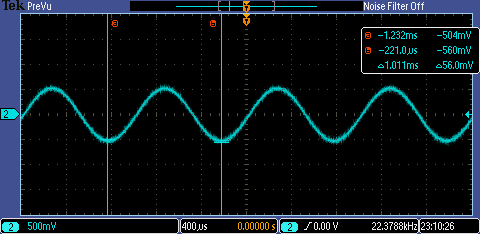
\includegraphics[width=\linewidth]{img/time_dom.png}
      \caption{Time Domain}
    \end{subfigure}

    \begin{subfigure}[b]{0.5\linewidth}
      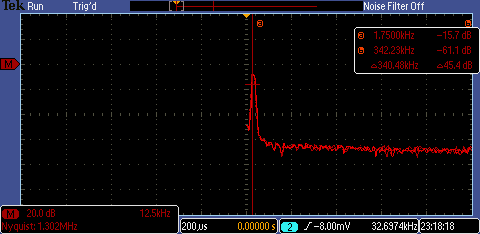
\includegraphics[width=\linewidth]{img/freq_dom.png}
      \caption{Frequency Domain}
    \end{subfigure}

  \caption{1kHz Sine wave}
  \end{center}
\end{figure}

 
%----------------------------------------------------------------------------------------
%	SECTION 2
%----------------------------------------------------------------------------------------

\section{Methods}

\begin{figure}[H]
  \begin{center}

    \begin{subfigure}[b]{0.5\linewidth}
      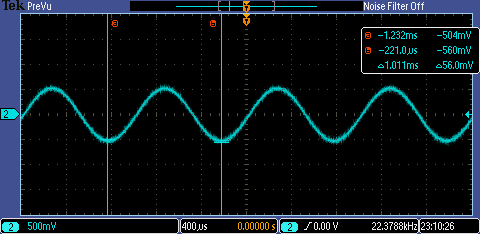
\includegraphics[width=\linewidth]{img/time_dom.png}
      \caption{Time Domain}
    \end{subfigure}

    \begin{subfigure}[b]{0.5\linewidth}
      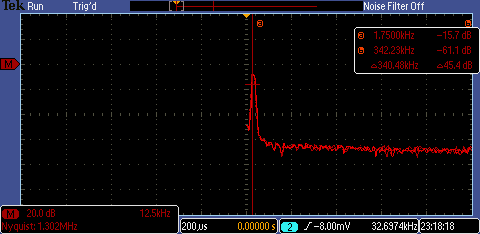
\includegraphics[width=\linewidth]{img/freq_dom.png}
      \caption{Frequency Domain}
    \end{subfigure}

  \caption{1kHz Sine wave}
  \end{center}
\end{figure}

 
%----------------------------------------------------------------------------------------
%	SECTION 3
%----------------------------------------------------------------------------------------

\section{Results}

\textbf{Code:}

\begin{verbatim}
  f = 5;
  t = (0:.001:1)';
  xt = sin(2*pi*f*t);

  %continous plot
  figure(1);
  plot(t,xt);
  xlabel('time');
  ylabel('amplitude');
  title('sine');

  %print values
  n = find(t == 0.32);
  xt(n)

  n = find(t == 0.64);
  xt(n)

  %sampled plot
  t = downsample(t, 8);
  xn = downsample(xt, 8);

  hold;
  stem(t, xn);

  %save to the report directory
  saveas(gcf, '../../report/lab_report_1/img/sine.png');
\end{verbatim}

\begin{figure}[h]
  \begin{center}
    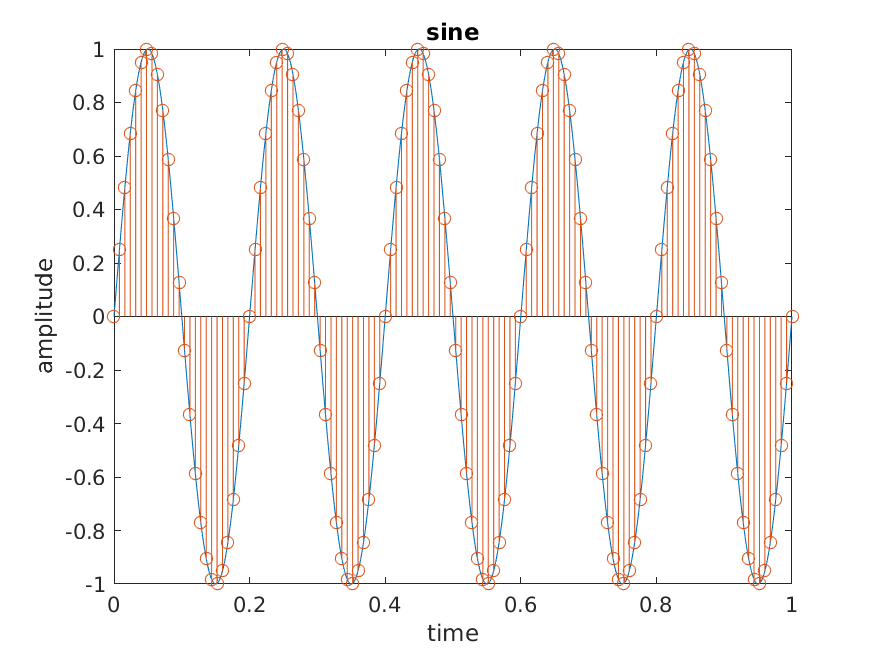
\includegraphics[width=0.65\textwidth]{img/sine.png}
    \caption{5Hz Sine wave.}
  \end{center}
\end{figure}


%----------------------------------------------------------------------------------------
%	SECTION 4
%----------------------------------------------------------------------------------------

\section{Answers to Lab Questions}

\begin{enumerate}
  \begin{item}
	  Draw the block diagram for the architecture of TMS320C671x core. Explain how this architecture allows for greater functional parallelism.\\

  \pagebreak
  \textbf{Answer:}
  \begin{figure}[H]
    \begin{center}
      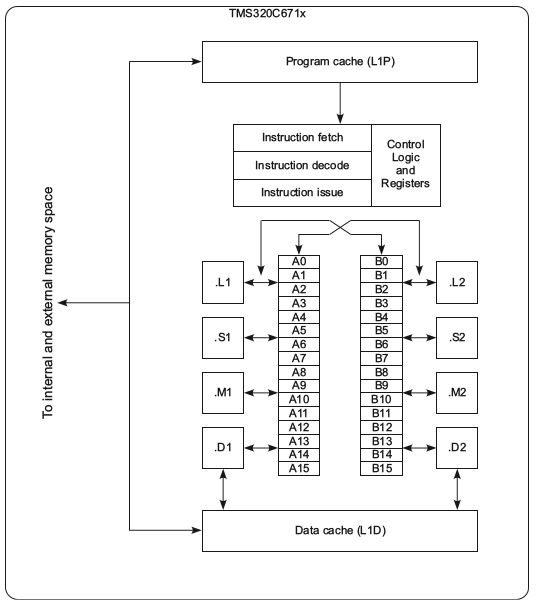
\includegraphics[width=0.4\textwidth]{img/core_arch.png}
      \caption{TMS320C671x architecture \cite{Welch:2011}.}
    \end{center}
  \end{figure}

    The core contains 8 functional units, each of these units is capable many different operations. 
    This allows us to perform two multiplies, and up to 4 arithmetic operations in parallel.

  \end{item}

  \begin{item}
    What is aliasing? How do you manage aliasing in DSP applications?

  \textbf{Answer:}
    Aliasing is when the high frequency content of your analog signal appears to be at a lower frequency in discrete time.
    To prevent aliasing in our applications we will filter the input signal with a lowpass filter that has a cutoff frequency of $\frac{f_s}{2}$.
  \end{item}

  \begin{item}
    Draw a block diagram of a generic DSP system and a talk-through system.

  \textbf{Answer:}
  \begin{figure}[H]
    \begin{center}

      \begin{subfigure}[b]{0.5\linewidth}
        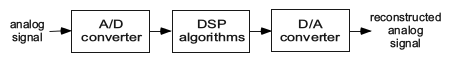
\includegraphics[width=\linewidth]{img/dsp.png}
        \caption{Generic DSP \cite{Welch:2011}.}
      \end{subfigure}

      \begin{subfigure}[b]{0.5\linewidth}
        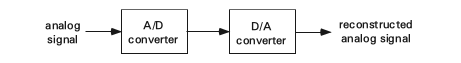
\includegraphics[width=\linewidth]{img/talk_thru.png}
        \caption{Talk Thru \cite{Welch:2011}.}
      \end{subfigure}

      \caption{DSP System.}
    \end{center}
  \end{figure}
  \end{item}

  \begin{item}
    Change the code in the “ISRs.c” file to implement: talk-through with swap (left channel; right channel). You don’t have to run the project or show the result. Just write down the necessary code.

  \textbf{Answer:}
    \begin{verbatim}
    float temp;

    temp = CodecData.channel[RIGHT];
    CodecData.channel[RIGHT] = CodecData.channel[LEFT];
    CodecData.channel[LEFT] = temp;
    \end{verbatim}
  \end{item}

  \begin{item}
    How are 32-bit floating-point results saved on the 'C6000 processors? Explain briefly the IEEE single-precision floating-point format. When does the 'C6000 use IEEE single-precision floating-point format (i.e give an example of an operation)

  \textbf{Answer:}
    32-bit floating point numbers are stored in IEEE single precision floating point format.
    IEEE format reserves one bit for sign, followed by 8 exponent bits, followed by 23 mantisa bits.
    The exponent is excess 127, and the mantisa is normalized so the leading bit is a one.
    The 'C6000 uses single precision when only floats are invloved i.e. ($1.0F + 1.0F$).
  \end{item}

  \begin{item}
    How does the scheduler work in DSP/BIOS?

  \textbf{Answer:}
    The scheduler periodically interrupts the current thread and determines what the highest priority thread is that is ready to execute.
  \end{item}

  \begin{item}
    What are the different threads present in DSP/BIOS? State the names in descending order of priority and describe in brief the function of each thread.

  \textbf{Answer:}
    Hardware Interrupt, triggered by hardware, used to transfer data or to trigger software interrupts.
    Software Interrupt, used to handle involved processing.
    Periodic Function, similar to software interrupt, but scheduled at regular intervals.
    Tasks, functions that handle the most complex processing.
    Idle Functions, used for system maintenance when there are no pending threads.
  \end{item}

  \begin{item}
    How will you determine the number of clock cycles required to execute your program?

  \textbf{Answer:}
    By changing the state of a logical signal upon entering and leaving my ISR, and monitoring that signal with an osciloscope.
  \end{item}

  \begin{item}
    How does an external processor access the entire memory space of the DSP?

  \textbf{Answer:}
    Using the enhanced direct memory access controller.
  \end{item}

  \begin{item}
    What is the purpose of the board support library?

  \textbf{Answer:}
    To standardize access to DSP hardware.
  \end{item}
\end{enumerate}

%----------------------------------------------------------------------------------------
%	BIBLIOGRAPHY
%----------------------------------------------------------------------------------------

\bibliography{mybib}
\bibliographystyle{plain}

%----------------------------------------------------------------------------------------


\end{document}
